%%%%%%%%%%%%%%%%%%%%%%%%%%%%%%%%%%%%%%%%%%%%%%%%%%%%%%%%%%%%%%%
%
% Welcome to writeLaTeX --- just edit your LaTeX on the left,
% and we'll compile it for you on the right. If you give
% someone the link to this page, they can edit at the same
% time. See the help menu above for more info. Enjoy!
%
%%%%%%%%%%%%%%%%%%%%%%%%%%%%%%%%%%%%%%%%%%%%%%%%%%%%%%%%%%%%%%%

% --------------------------------------------------------------
% This is all preamble stuff that you don't have to worry about.
% Head down to where it says "Start here"
% --------------------------------------------------------------
 
\documentclass[12pt]{report}
 
\usepackage[margin=1in]{geometry}
\usepackage{amsmath,amsthm,amssymb}
\usepackage{hyperref}
\usepackage[nottoc,numbib]{tocbibind}
\usepackage{graphicx}
\graphicspath{{./images/}}

\usepackage{listings}
\usepackage{xcolor}

%New colors defined below
\definecolor{codegreen}{rgb}{0,0.6,0}
\definecolor{codegray}{rgb}{0.5,0.5,0.5}
\definecolor{codepurple}{rgb}{0.58,0,0.82}
\definecolor{backcolour}{rgb}{0.95,0.95,0.92}

%Code listing style named "mystyle"
\lstdefinestyle{mystyle}{
  backgroundcolor=\color{backcolour}, commentstyle=\color{codegreen},
  keywordstyle=\color{magenta},
  numberstyle=\tiny\color{codegray},
  stringstyle=\color{codepurple},
  basicstyle=\ttfamily\footnotesize,
  breakatwhitespace=false,         
  breaklines=true,                 
  captionpos=b,                    
  keepspaces=true,                 
  numbers=left,                    
  numbersep=5pt,                  
  showspaces=false,                
  showstringspaces=false,
  showtabs=false,                  
  tabsize=2
}

%"mystyle" code listing set
\lstset{style=mystyle}

 
\newcommand{\N}{\mathbb{N}}
\newcommand{\Z}{\mathbb{Z}}
 
\newenvironment{theorem}[2][Theorem]{\begin{trivlist}
\item[\hskip \labelsep {\bfseries #1}\hskip \labelsep {\bfseries #2.}]}{\end{trivlist}}
\newenvironment{lemma}[2][Lemma]{\begin{trivlist}
\item[\hskip \labelsep {\bfseries #1}\hskip \labelsep {\bfseries #2.}]}{\end{trivlist}}
\newenvironment{exercise}[2][Exercise]{\begin{trivlist}
\item[\hskip \labelsep {\bfseries #1}\hskip \labelsep {\bfseries #2.}]}{\end{trivlist}}
\newenvironment{problem}[2][Problem]{\begin{trivlist}
\item[\hskip \labelsep {\bfseries #1}\hskip \labelsep {\bfseries #2.}]}{\end{trivlist}}
\newenvironment{question}[2][Question]{\begin{trivlist}
\item[\hskip \labelsep {\bfseries #1}\hskip \labelsep {\bfseries #2.}]}{\end{trivlist}}
\newenvironment{corollary}[2][Corollary]{\begin{trivlist}
\item[\hskip \labelsep {\bfseries #1}\hskip \labelsep {\bfseries #2.}]}{\end{trivlist}}

\newenvironment{solution}{\begin{proof}[Solution]}{\end{proof}}
 
\begin{document}
 
% --------------------------------------------------------------
%                         Start here
% --------------------------------------------------------------
 
\title{Texas A\&M University Kingsville\\
Department of EECS\\
CSEN 5322 Operating Systems\\
Assignment 1 Matrix Multiplication
}%Institution, Department
\author{\\
Mengxiang Jiang %replace with your name
} %if necessary, replace with your course title
 
\maketitle

\tableofcontents

\chapter{Introduction}
Matrix multiplication has a huge number of applications in not just computer science but almost every technical field, 
ranging from computer graphics and neural networks to Markov chains used in both quantum mechanics and economics. As such,
a huge amount of research has been done to efficiently do it. One might think the time complexity $\Theta(n^3)$ bounds the number of scalar multiplications needed, but
Strassen's runs in $\Theta(n^{\lg{7}})$ or about $O(n^{2.81})$ time.\cite{clrs} This is by no means the best algorithm, and it is still an open problem what the optimal time complexity is.
In fact, Deep Mind recently published a paper about using reinforcement learning to reduce the number of scalar multiplications for this purpose.\cite{Fawzi2022}
However, in this assignment, I am not going to use one of the more advanced algorithms but instead parallelize the naive algorithm,
thereby taking advantage of hardware. The programming language I will use is C and the main library to parallelize the computation is MPI.

\chapter{Design}
Originally, I intended to send a single row and a single column from the input matrices to each process to compute each entry of the output matrix independently.
However, after doing this and testing the performance, it was significantly worse than not parallelizing the code at all, so instead, I decided to use the implementation
given by the Lawrence Livermore National Laboratory MPI tutorial.\cite{llnl} The way this implementation works is by having a master process divide the number of rows
in input matrix by the number workers and sending each worker that many rows of A. 
If the two numbers do not evenly divide, then the extra rows are sent to each worker until no extra are left. Next, the entire input matrix B is sent to all the workers.
Then the workers uses the naive matrix multiplication algorithm to calculate an intermediate output matrix and sends it to the master, who puts it together in the output matrix C.
Below is a picture of how this works for a 5x3 matrix times a 3x2 matrix:

\begin{figure}[ht]
    \centering
    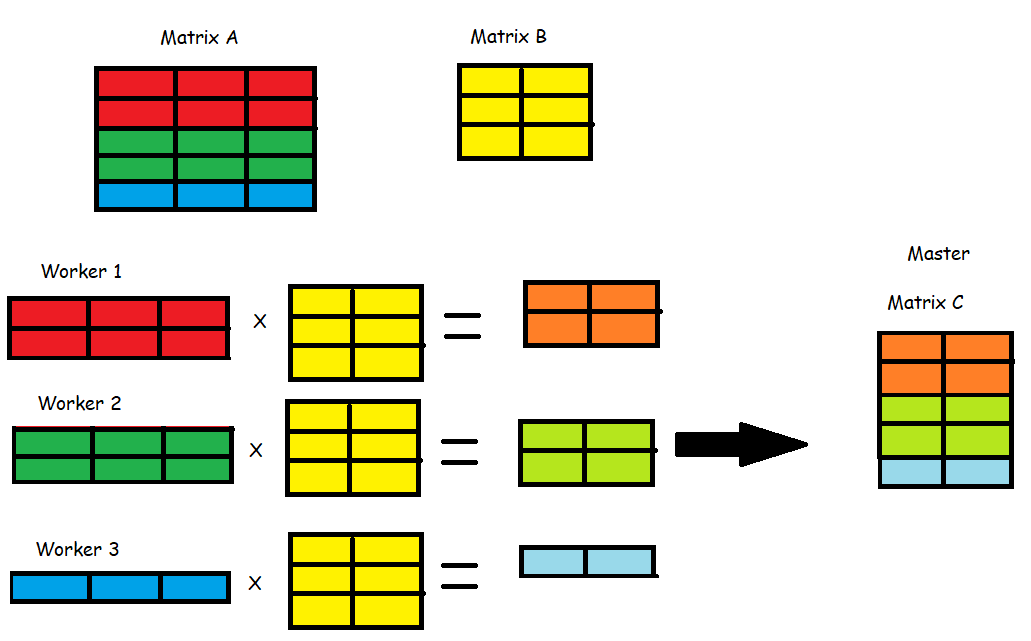
\includegraphics[scale=0.5]{algorithm}
    \caption{distributive algorithm}
\end{figure}

\chapter{Results}
Running the read from file write to file matrix multiplication code (matrixmul.c) with 4 processes (1 master 3 workers) gives the following results:
\begin{lstlisting} [language=C, caption=terminal1.txt]
$ mpicc matrixmul.c -o matrixmul
$ mpirun -np 4 ./matrixmul input0.txt
mpi_mm has started with 4 tasks.
Initializing matrices...
Number of Rows of A: 3
Number of Columns of A (also Rows of B): 4
Number of Columns of B: 5

Matrix A:

    3.45    -5.12     2.06   -19.10
    1.23     0.90     6.20    10.00
    9.57     9.01    -2.06     2.39
******************************************************

Matrix B:

    5.43   -12.50    65.02    -1.10     6.20
    3.21    -9.02     4.56   -11.22     4.01
    5.82     1.08    -2.06   -23.45   -13.72
    83.47    56.10     4.28    42.20    -2.34
******************************************************
Sending 1 rows to task 1 offset=0
Sending 1 rows to task 2 offset=1
Sending 1 rows to task 3 offset=2
Received results from task 1
Received results from task 2
Received results from task 3
******************************************************
Result Matrix:

-1580.01   -1066.23   114.94   -800.58    17.34
880.35   544.20   114.16   265.16   -97.23
268.41   -69.04   677.79    37.45   118.08
******************************************************
Done.
wall clock time = 0.003205
\end{lstlisting}

Note that the total time (0.003205 seconds) is longer than a sequential multiplication on random matrices of size 100x100 (0.001178 seconds).
This is likely due to reading and writing to file, which is incredibly slow in comparison.

For the random nxn square matrix multiplication, I increased the maximum n from 50 to 500 because 50x50 was too small to notice.
I also decreased the number of executions from 100 iterations to 10 iterations since the average times didn't seem to change much.
For parallel execution, I did multiple runs with number of workers ranging from 2 to 8. Below is the plot of the results:

\begin{figure}[ht]
    \centering
    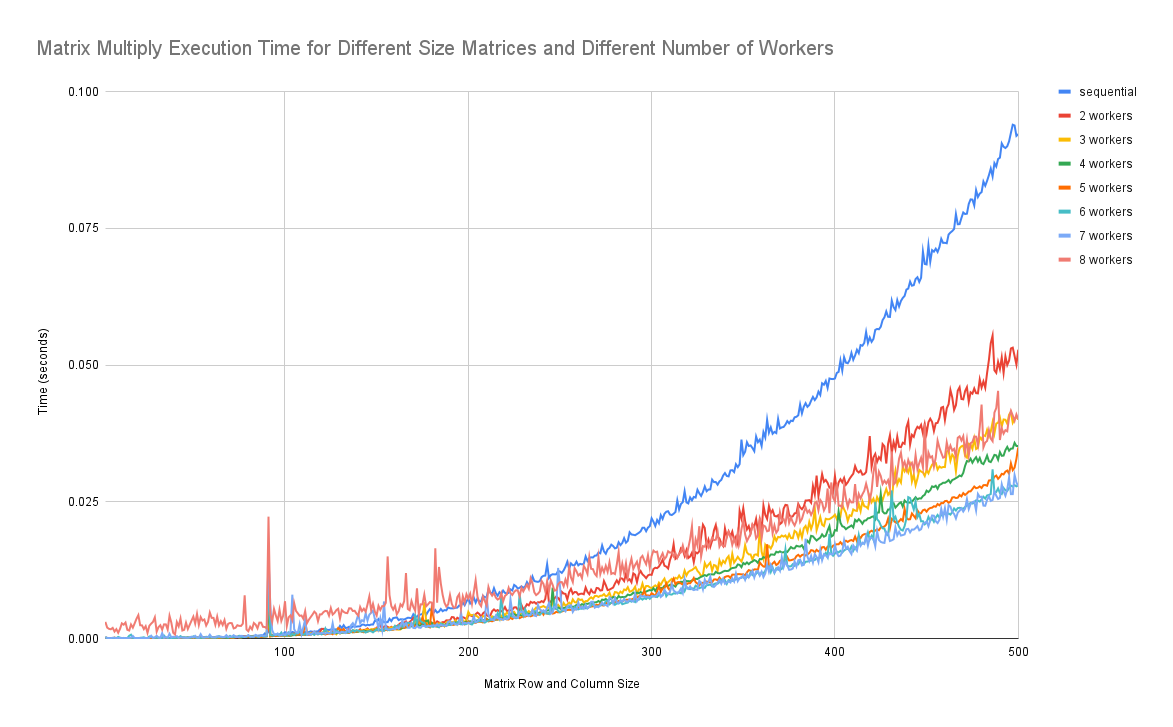
\includegraphics[width=\textwidth]{avgtimes}
    \caption{execution times}
\end{figure}

The biggest performance gain is from sequential to 2 workers. Every additional worker saw less gain, and when at 8 workers, there was a performance loss,
very likely due to my computer having only 4 cores and 8 logical processors. Below is a copy paste of my dxdiag report:
\pagebreak
\begin{verbatim}
    ------------------
    System Information
    ------------------
          Time of this report: 10/19/2022, 02:44:00
                 Machine name: DESKTOP-25GTGVH
                   Machine Id: {9D8D4EA9-61DB-4C7A-BB3A-78BEF6E203AB}
             Operating System: Windows 10 Pro 64-bit (10.0, Build 19043) (19041.vb_release.191206-1406)
                     Language: English (Regional Setting: English)
          System Manufacturer: ASUS
                 System Model: All Series
                         BIOS: 2205 (type: UEFI)
                    Processor: Intel(R) Core(TM) i7-4790K CPU @ 4.00GHz (8 CPUs), ~4.0GHz
                       Memory: 16384MB RAM
          Available OS Memory: 16260MB RAM
                    Page File: 23200MB used, 6371MB available
                  Windows Dir: C:\WINDOWS
              DirectX Version: DirectX 12
          DX Setup Parameters: Not found
             User DPI Setting: 96 DPI (100 percent)
           System DPI Setting: 96 DPI (100 percent)
              DWM DPI Scaling: Disabled
                     Miracast: Available, no HDCP
    Microsoft Graphics Hybrid: Not Supported
     DirectX Database Version: 1.0.8
               DxDiag Version: 10.00.19041.2075 64bit Unicode
\end{verbatim}

Note I am using Windows Subsytem for Linux using Ubuntu 14.04.6 LTS trusty with mpich version 3.0.4 when running these programs.

\bibliographystyle{plain}
\bibliography{refs}

% --------------------------------------------------------------
%     You don't have to mess with anything below this line.
% --------------------------------------------------------------
 
\end{document}